\section{Coding Guidelines}

\mult{2}

\begin{remark}
    \begin{itemize}
        \item reduce the number of bugs
        \item robustness
        \item correctness
        \item maintainability
        \item facilitate code reading within a team
        \item takes less time to understand another team member's code
        \item improve portability   
        \item reuse of code on other HW platforms
    \end{itemize}
    \textbf{Enforce by}
    \begin{itemize}
        \item automated scans (part of static code checking)
        \item peer reviews
    \end{itemize}
\end{remark}

\begin{definition}{Appearance}
    \begin{itemize}
        \item Indentation: 4 spaces (no tabs)
        \item Line length: 80 characters
        \item Only one statement per line (readability)
        \item No trailing whitespace (no spaces at the end of a line)
        \item Parentheses to aid clarity (do not rely on operator precedence)
        \item No magic numbers (use constants instead)
    \end{itemize}
\end{definition}

\multend

\subsubsection{Braces}

\mult{2}

\begin{definition}{Non-function statement blocks}
    \texttt{if, else, while, for, do, do-while, switch}
    \\
    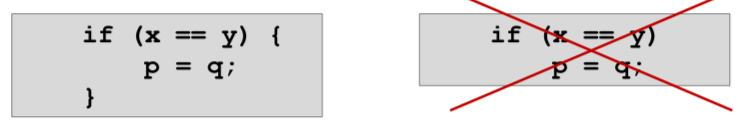
\includegraphics[width=\linewidth]{braces_nonfunctionstatements.png}
    \\
    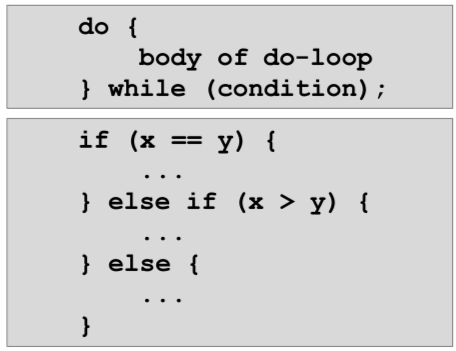
\includegraphics[width=\linewidth]{closing_braces.png}
\end{definition}

\begin{definition}{Function statement blocks}
    \texttt{function, class, namespace}
    \\
    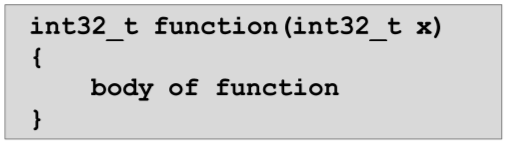
\includegraphics[width=\linewidth]{braces_functions.png}
    \\
    \texttt{struct, enum:}
    \\
    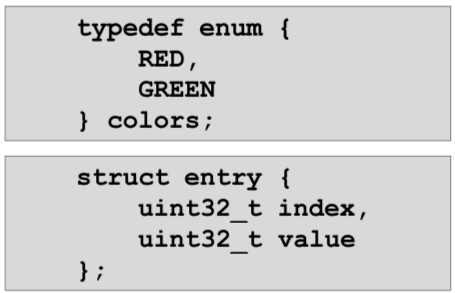
\includegraphics[width=\linewidth]{braces_struct_enum.png}
\end{definition}

\multend

\subsubsection{Spaces}

\mult{2}

\begin{remark}
    \begin{itemize}
    \item Mostly function-versus-keyword usage Use space after keywords
    \texttt{if, switch, case, for, do, while}
    \item No space with sizeof, typeof, alignof, or attribute (as they look somewhat like functions)
    \\ \texttt{s = sizeof(struct file);}
    \item Pointer declaration: * adjacent to data name or function name
    \\ \texttt{uint8\_t *ptr;}
    \\ \texttt{uint32\_t parse(uint8\_t *ptr, uint8\_t **retptr);}
    \\ \texttt{uint8\_t *match(uint8\_t *s);}
    \end{itemize}
\end{remark}

\begin{definition}{Operators}
    \begin{itemize}
        \item No space before or after unary operators: ++, --, +, -, !, ~, \texttt{(type), (cast), sizeof, typeof, alignof, \_attribute\_, defined}
        \item One space before or after binary/ternary operators: *, /, \%, +, -, <<, >>, <, <=, >, >=, ==, !=, ?, :
        \item No space around struct member operator: . and ->
        \item No trailing whitespaces!
    \end{itemize}
\end{definition}

\multend

\subsubsection{Functions}

\mult{2}

\begin{remark}
    \begin{itemize}
        \item short and sweet (less than 50 lines)
        \item do just one thing
        \item no more than 5-10 local variables
        \item no more than 3 parameters
        \item function prototypes shall include parameter names with their data types
        \item no more than 3 levels of indentation (if, for, while, do-while)
        \item no more than 2 nested loops (for, while, do-while)
    \end{itemize}
\end{remark}

\begin{definition}{Function Parameters}
    Use const to define call-by-reference function parameters that should not be modified
- int32\_t strlen (const int8\_t s[]);
strlen() does not modify any character of character array s
- void display(mystruct const *param) ;
\end{definition}

\begin{definition}{Function Definition}
Just one exit point and it shall be at the bottom of the function
- keyword return shall appear only once
- All 'private' functions shall be defined static
- 'private' $\rightarrow$ Functions that are only used within the module itself. The function is an implementation detail and not accessible from other modules
A prototype shall be defined for each 'public' function in the module header file module.h
- 'public' $\rightarrow$ Functions that are called by other modules. The function prototypes are part of the module interface.
\end{definition}

\begin{definition}{Return Values}
    Shall be checked by the caller
If the name of a function is an action or an imperative command
- Function should return an error-code integer i.e. 0 for success and -Exxx for failure.
- If possible error codes shall be based on the Posix Errorcode
- If self-defined error codes are being used they shall be properly documented. In the header file for public functions or in the .c file for private functions
- For example, "add work" is a command, and the add\_work () function returns 0 for success or -EBUSY for failure.

If the name of a function is a predicate
- Function should return a "succeeded" boolean.
- "PCI device present" is a predicate, and the pci\_dev\_present () function returns 1 if it succeeds in finding a matching device or 0 if it doesn't.
- Functions whose return value is the actual result of a computation, rather than an indication of whether the computation succeeded, are not subject to this rule.
- Generally they indicate failure by returning some out-of-range result.
- Typical examples would be functions that return pointers; they use NULL or the ERR\_PTR mechanism to report failure.
\end{definition}

\multend

\subsubsection{General Rules}

\mult{2}

\begin{definition}{Naming}
No macro name (\#define) shall contain any lowercase letters
- Function and variable names shall not contain uppercase letters
- Use descriptive names for functions, global variables and important local variables
- Underscores shall be used to separate words in names e.g. count\_active\_users()
Use short names e.g. i for auxiliary local variables like loop counters
- Do not encode types in names. Let the compiler do the type checking
\end{definition}

\begin{definition}{Comments}
    - All comments shall be in English
- C99 comments // are allowed
- Explain WHAT your code does not HOW
- Don't repeat what the statement says in a comment.
- Assume that the reader is familiar with C
- Comments shall never be nested
- All assumptions shall be spelled out in comments
- or even better in a set of design-by-contract tests or assertions
- The interface of a public function shall be commented next to the function prototype in the header file.
- The comment shall not be repeated next to the function definition in the .c file
\end{definition}

\begin{definition}{Types}
    - Use fixed width C99 data types from stdint. h
    - e.g. uint8\_t or int32\_t rather than unsigned char or int
    - Type char shall be restricted to declarations and operations on strings
    - Bit-fields shall not be defined within signed integer types
    - None of the bit-wise operators shall be used to manipulate signed integer data
    %- i.e. do not use $\&, |, ~, ^, <<, >>$ on signed integers

    Signed integers shall not be combined with unsigned integers in comparisons or expressions
- Decimal constants meant to be unsigned should be declared with an ' $U$ ' at the end
Casts shall be done explicitly and accompanied by a comment
- Use just one data declaration or one data definition per line
- Allows a comment for each item.
\end{definition}

\begin{definition}{Header Files}
    There shall be precisely one header file for each module
Each header file shall contain a preprocessor guard against multiple inclusion
\texttt{
\#ifndef \_ADC\_H \\
\#define \_ADC\_H \\
\#endif /* \_ADC\_H */
}

Only add \#includes that are immediately needed for this header file; do not add \#includes for convenience of others
Do not define or declare variables
- i.e. uint32\_t count / extern uint32\_t count

\end{definition}

\multend

\subsection{Coding Techniques}

\begin{example2}{Example: Module Traffic Light}
    \\
    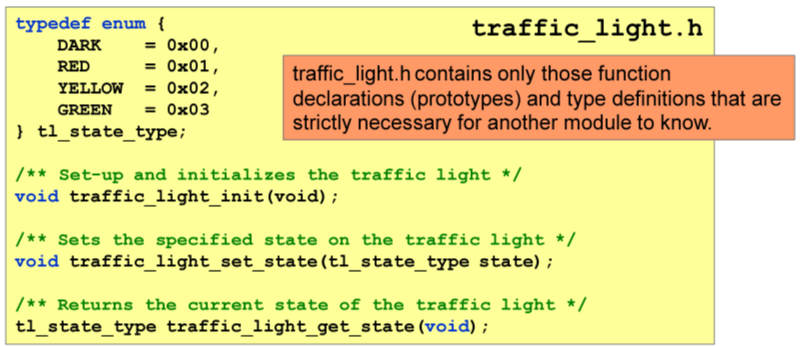
\includegraphics[width=\linewidth]{module_traffic_light_h.png}
    \\
    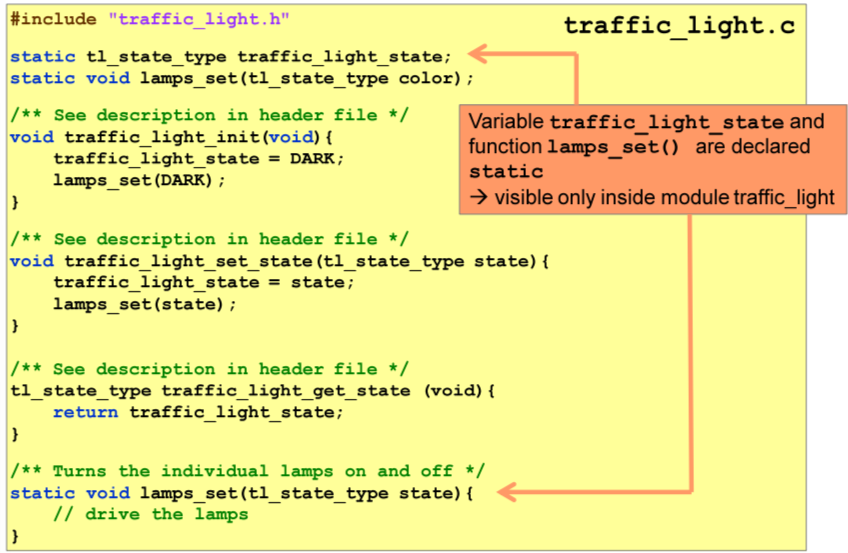
\includegraphics[width=\linewidth]{module_traffic_light_c.png}
\end{example2}

\mult{2}

\begin{remark}
    Encapsulation:
    \begin{itemize}
        \item Interface: .h file
        \item Implementation: .c file
    \end{itemize}
\end{remark}

\begin{remark}
    \textcolor{pink}{maybe finish but not rn}
\end{remark}

\multend

